\documentclass[a4paper, 12pt,twoside]{book}

% set the paper size and the margins
\usepackage[top = 2cm, bottom = 2cm, left = 2cm, right = 4cm ]{geometry}
\usepackage[showboxes]{textpos}
\setlength{\TPHorizModule}{10mm}
\setlength{\TPVertModule}{\TPHorizModule}
\TPMargin{2mm}
% set the header and the footnote
\usepackage{fancyhdr}
% Supress the hyphenation
\hyphenation{thatshouldnot}
% for table and equations
\usepackage{tablefootnote}
\usepackage{amsmath,amsfonts,amsthm}
\usepackage{multirow}
\usepackage{hhline}
% make a wide hat for the least-squares regression line
 \usepackage{scalerel,stackengine}
\stackMath
\newcommand\reallywidehat[1]{%
\savestack{\tmpbox}{\stretchto{%
  \scaleto{%
    \scalerel*[\widthof{\ensuremath{#1}}]{\kern-.6pt\bigwedge\kern-.6pt}%
    {\rule[-\textheight/2]{1ex}{\textheight}}%WIDTH-LIMITED BIG WEDGE
  }{\textheight}% 
}{0.5ex}}%
\stackon[1pt]{#1}{\tmpbox}%
}
\usepackage[shortlabels]{enumitem}

% knitr packages
\usepackage[]{graphicx}
\usepackage[]{color}
%% maxwidth is the original width if it is less than linewidth
%% otherwise use linewidth (to make sure the graphics do not exceed the margin)
\makeatletter
\def\maxwidth{ %
  \ifdim\Gin@nat@width>\linewidth
    \linewidth
  \else
    \Gin@nat@width
  \fi
}
\makeatother

\definecolor{fgcolor}{rgb}{0.345, 0.345, 0.345}
\newcommand{\hlnum}[1]{\textcolor[rgb]{0.686,0.059,0.569}{#1}}%
\newcommand{\hlstr}[1]{\textcolor[rgb]{0.192,0.494,0.8}{#1}}%
\newcommand{\hlcom}[1]{\textcolor[rgb]{0.678,0.584,0.686}{\textit{#1}}}%
\newcommand{\hlopt}[1]{\textcolor[rgb]{0,0,0}{#1}}%
\newcommand{\hlstd}[1]{\textcolor[rgb]{0.345,0.345,0.345}{#1}}%
\newcommand{\hlkwa}[1]{\textcolor[rgb]{0.161,0.373,0.58}{\textbf{#1}}}%
\newcommand{\hlkwb}[1]{\textcolor[rgb]{0.69,0.353,0.396}{#1}}%
\newcommand{\hlkwc}[1]{\textcolor[rgb]{0.333,0.667,0.333}{#1}}%
\newcommand{\hlkwd}[1]{\textcolor[rgb]{0.737,0.353,0.396}{\textbf{#1}}}%
\let\hlipl\hlkwb
\usepackage{framed}
\makeatletter
\newenvironment{kframe}{%
 \def\at@end@of@kframe{}%
 \ifinner\ifhmode%
  \def\at@end@of@kframe{\end{minipage}}%
  \begin{minipage}{\columnwidth}%
 \fi\fi%
 \def\FrameCommand##1{\hskip\@totalleftmargin \hskip-\fboxsep
 \colorbox{shadecolor}{##1}\hskip-\fboxsep
     % There is no \\@totalrightmargin, so:
     \hskip-\linewidth \hskip-\@totalleftmargin \hskip\columnwidth}%
 \MakeFramed {\advance\hsize-\width
   \@totalleftmargin\z@ \linewidth\hsize
   \@setminipage}}%
 {\par\unskip\endMakeFramed%
 \at@end@of@kframe}
\makeatother


\definecolor{shadecolor}{rgb}{.97, .97, .97}
\definecolor{messagecolor}{rgb}{0, 0, 0}
\definecolor{warningcolor}{rgb}{1, 0, 1}
\definecolor{errorcolor}{rgb}{1, 0, 0}
\newenvironment{knitrout}{}{} % an empty environment to be redefined in TeX

\usepackage{alltt}


% packages will be used by the 'kable' package
\usepackage{booktabs}
\usepackage{longtable}
\usepackage{array}
\usepackage{multirow}
\usepackage[table]{xcolor}
\usepackage{wrapfig}
\usepackage{float}
\usepackage{colortbl} 
\usepackage{pdflscape}
\usepackage{tabu}
\usepackage{threeparttable}
\usepackage{threeparttablex}
\usepackage[normalem]{ulem}
%\usepackage{makecell}
\usepackage{xcolor}
\IfFileExists{upquote.sty}{\usepackage{upquote}}{}

% define a color for highlight
\definecolor{asparagus}{rgb}{0.53, 0.66, 0.42}
\definecolor{babypink}{rgb}{0.96, 0.76, 0.76}
\definecolor{champagne}{rgb}{0.97, 0.91, 0.81}
\definecolor{forestgreen}{rgb}{0.13, 0.55, 0.13}
\definecolor{dollarbill}{rgb}{0.52, 0.73, 0.4}

\usepackage{tcolorbox}

\tcbset{width=0.9\textwidth,boxrule=0pt,colback=champagne,arc=0pt,
auto outer arc,left=0pt,right=0p}

\setlength{\parindent}{0cm}
\begin{document}

%Deal with the headers of each chapter
\pagestyle{fancy}
\fancyhf{}
\renewcommand{\chaptermark}[1]{ \markboth{#1}{} }
\fancyhead[CE,CO]{\leftmark}
\fancyfoot[LE,RO]{\thepage}

\chapter{One-variable data analysis}
\thispagestyle{empty}
In this chapter, we start with the simplest case, where there is only one variable. We will learn some basic concepts and how to describe the data both numerically and graphically. Some more advanced concepts, such as density curve, normal distribution are also introduced.
\newpage

\begin{center}
\begin{knitrout}
\definecolor{shadecolor}{rgb}{0.969, 0.969, 0.969}\color{fgcolor}
\rowcolors{2}{gray!6}{white}

\begin{table}[!h]
\caption{\label{ExampleData}Example Data\tablefootnote{MID is the scores in the midterm exam. FINAL is the scores in the final exam. BASKETBALL indicates whether a student plays basketball or not.}}
\centering
\scalebox{0.8}{
\begin{tabular}[t]{cccccc}
\hiderowcolors
\toprule
 NAME& CLASS & GENDER & MID & FINAL & BASKETBALL\\
\midrule
\showrowcolors
James & 23 & M & 74 & 86 & N\\
Andrew & 23 & M & 74 & 86 & Y\\
Jim & 23 & M & 23 & 47 & Y\\
Kim & 23 & M & 61 & 78 & Y\\
Mark & 23 & M & 97 & 98 & N\\
Owen & 23 & M & 73 & 85 & Y\\
Cook & 23 & M & 98 & 99 & Y\\
Albert & 23 & M & 81 & 90 & Y\\
Donald & 23 & M & 70 & 84 & N\\
Peter & 23 & M & 53 & 72 & Y\\
Vince & 23 & M & 68 & 82 & Y\\
Davis & 23 & M & 83 & 91 & Y\\
Alan & 23 & M & 82 & 90 & Y\\
Nick & 23 & M & 64 & 80 & N\\
Elina & 23 & F & 72 & 85 & N\\
Daisy & 23 & F & 68 & 82 & Y\\
Crystal & 23 & F & 53 & 72 & N\\
Karida & 23 & F & 66 & 81 & N\\
Linda & 23 & F & 83 & 91 & N\\
Dale & 23 & F & 70 & 83 & Y\\
Sandy & 23 & F & 56 & 74 & N\\
Emma & 23 & F & 65 & 80 & N\\
Angela & 23 & F & 72 & 85 & N\\
Katie & 23 & F & 84 & 91 & N\\
Eileen & 23 & F & 73 & 85 & N\\
Meggie & 23 & F & 68 & 82 & N\\
Jack & 24 & M & 45 & 67 & Y\\
Stan & 24 & M & 23 & 47 & Y\\
Ryan & 24 & M & 60 & 77 & Y\\
Murphy & 24 & M & 36 & 60 & N\\
Mike & 24 & M & 82 & 90 & Y\\
Antony & 24 & M & 18 & 42 & Y\\
Clare & 24 & M & 86 & 93 & Y\\
David & 24 & M & 83 & 91 & Y\\
Taylor & 24 & M & 69 & 83 & Y\\
Park & 24 & M & 78 & 88 & N\\
Gary & 24 & M & 51 & 71 & Y\\
Carson & 24 & M & 85 & 92 & Y\\
Elvis & 24 & M & 25 & 49 & Y\\
Kelly & 24 & F & 59 & 76 & N\\
Sara & 24 & F & 77 & 88 & N\\
Cherry & 24 & F & 61 & 78 & N\\
Lucy & 24 & F & 54 & 73 & Y\\
Hellen & 24 & F & 46 & 68 & N\\
Chloe & 24 & F & 95 & 97 & Y\\
Dorothy & 24 & F & 82 & 90 & N\\
Natalie & 24 & F & 73 & 85 & N\\
Vivien & 24 & F & 76 & 87 & N\\
Cathy & 24 & F & 70 & 84 & N\\
Carol & 24 & F & 55 & 74 & N\\
Bella & 24 & F & 96 & 98 & Y\\
Veronica & 24 & F & 60 & 77 & N\\
\bottomrule
\end{tabular}
}
\end{table}

\rowcolors{2}{white}{white}
\end{knitrout}
\end{center}
\section{Basic concepts}
\begin{itemize}
\item In  table \ref{ExampleData}, each student is an \textbf{individual}.
\item All students are described through perspectives of \textit{NAME, CLASS, GENDER, MID, FINAL,} and \textit{BASKETBALL}. Those different perspectives are called \textbf{variables}, for they may take different values for different students.
\item The values of \textit{MID} and \textit{FINAL} can be operated on like normal numbers, such as taking average, subtraction. Those variables are called 
\textbf{quantitative variables}.
\item The values of \textit{NAME, CLASS, GENDER} and \textit{BASKETBALL} only play the role of sorting individuals into different categories. Those variables are called \textbf{categorical variables}
\item The way a variable takes different values is called the \textbf{distribution} of this variable.
\item All the individuals we want to study is called the \textbf{population}.
\item A subset of the population is called a \textbf{sample}.

\colorbox{babypink}{Samples and populations are relative.} If you take all the Chinese people as the population, people in Shanghai is a sample. If you take all the people of the whole world as the population, then Chinese people is a sample.
\item The number of individuals in the sample is called the \textbf{sample size}.

\end{itemize}

\colorbox{babypink}{\parbox{14.2cm}{A variable takes values of numbers doesn't mean it is quantitative variable. }}

\begin{textblock}{3}(15.5, -3)
\textblockcolor{dollarbill}
Is \textit{CLASS} a quantitative or categorical variable?
\end{textblock}
\vspace{0.6cm}
\newpage

\section{Graphs to describe categorical variables}

\begin{itemize}

\item \textbf{Pie chart}\vspace{0.3cm}\\
There are 25 girls and 27 boys in table \ref{ExampleData}. The pie chart of the  distribution of \textit{GENDER} is given by figure \ref{piechart}.
  \begin{center}
    \begin{figure}[!htb]
     \centering
    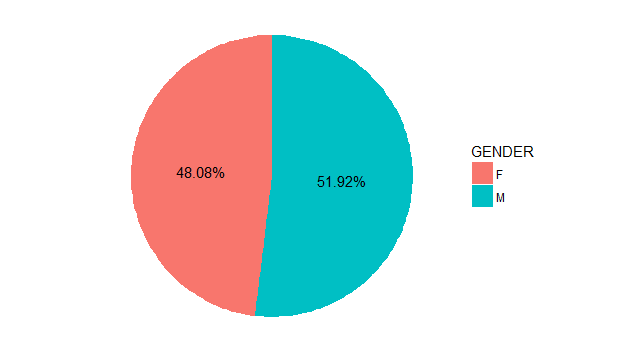
\includegraphics[scale=0.35]{PieChart.png}
    \caption{Pie chart of the distribution of the \textit{GENDER} }
    \label{piechart}
    \end{figure}  
\end{center} 

\item \textbf{Bar graph}\vspace{0.3cm}

Similarly, we can draw bar graph to show the information about \textit{GENDER}
    \begin{figure}[H]
      \centering
        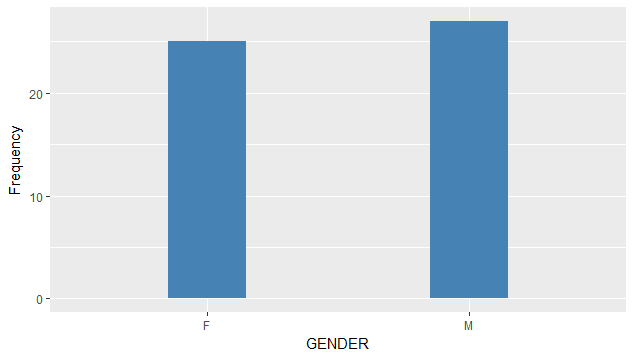
\includegraphics[scale=0.4]{Bargraph1.png}
        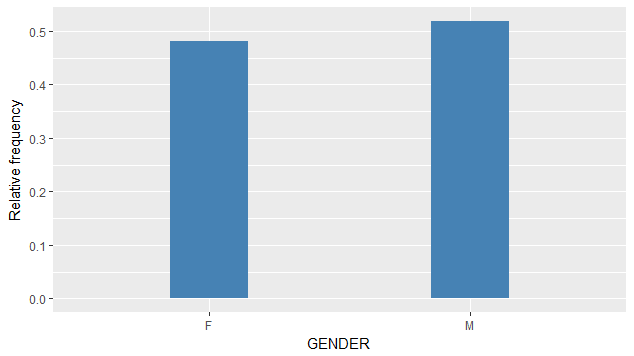
\includegraphics[scale=0.4]{Bargraph2.png}       
          \caption{Bar graphs with percentage and frequency as vertical axis} 
          \label{bargraph}
    \end{figure}    
 In figure \ref{bargraph}, the vertical axes are \textbf{frequency} and  \textbf{percentage} or (\textbf{relative frequency}) respectively. When the sample size is too big, it is better to use relative frequency as the vertical axis.\vspace{0.6cm}\\
\colorbox{babypink}{\parbox{14.2cm}{Be sure to label the axes whenever a graph is drawn!}}

\end{itemize}
\newpage

\section{{Graphs to describe Quantitative Variables}}

 \begin{itemize}

\item \textbf{Dotplot}\\
\begin{figure}[H]
\centering
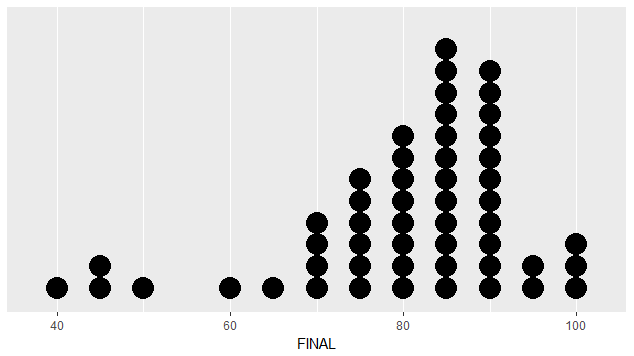
\includegraphics[scale=0.3]{Dotplot.png}
\caption{Dotplot of the distribution of the \textit{FINAL}}
\label{dotplot}
\end{figure}

\noindent In figure \ref{dotplot}, the \textbf{bin width} is 5. For example, there is only one score lies in the interval $(37.5, 42.5]$, which is "42" from the student whose name is "Antony", and the width of this interval is $42.5-37.5 = 5$, which is the bin width. Similarly, there are eight scores lies in the interval $(77.5, 82.5]$. 
\vspace{0.6cm}

\item \textbf{Stemplot}\vspace{0.3cm}

The \textbf{stemplot} is also called \textbf{stem-leaf plot}, as shown in figure \ref{Stemplot}. The numbers to the left side of the vertical line are the "stems", and the numbers to the right side of the vertical line are the leaves.
\begin{figure}[H]
\centering
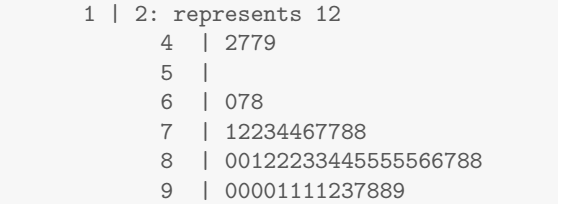
\includegraphics[scale=0.6]{Stemplot.png}
\caption{The stemplot for the \textit{FINAL}}
\label{Stemplot}
\end{figure}
\begin{textblock}{5}(13, -3)
\textblockcolor{dollarbill}
\noindent Can we erase the empty stem? 
\end{textblock}
\noindent Sometimes the leaves are too long, we have to split them, and this type of stemplot is the steamplot with \textbf{splitting stems}. As shown in figure \ref{StemplotSplittingStems}, each stem splits into two stems. The first stem holds digits from 0 to 4, the second from 5 to 9. They hold the same number of digits.
\begin{figure}[H]
\centering
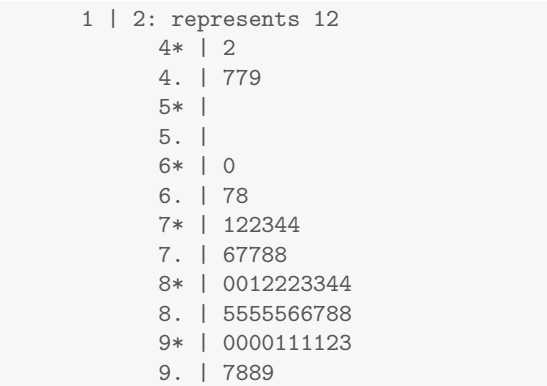
\includegraphics[scale=0.6]{StemplotSplittingStems.png}
\caption{The stemplot with splitting stems for the \textit{FINAL}}
\label{StemplotSplittingStems}
\end{figure}
\begin{textblock}{5}(13, -5)
\textblockcolor{dollarbill}
\noindent Why should each stem hold the same number of digits? 
\end{textblock}
\vspace{0.6cm}
\newpage

\item \textbf{Histogram}\vspace{0.3cm}

If the dots in dotplot is replaced by bars, the graph will be histogram, as shown in figure 

\begin{figure}[H]
\centering
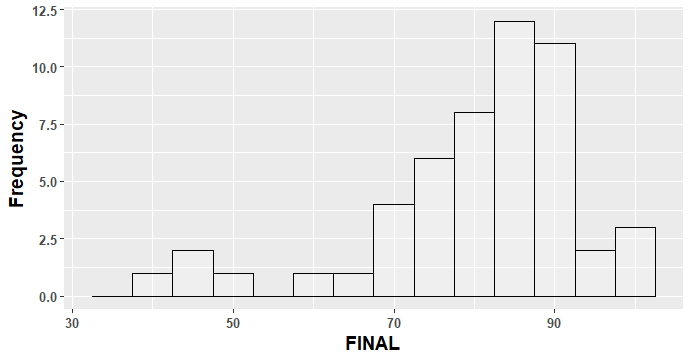
\includegraphics[scale=0.4]{Histogram1.png}
\caption{Histogram of the distribution of the \textit{FINAL}}
\label{HistogramFrequency}
\end{figure}

\begin{textblock}{4.8}(-3, -4.5)
\textblockcolor{dollarbill}
 What is the difference between histogram and bar graph?
 \end{textblock}
 
The vertical axis can be relative frequency as well.
\begin{figure}[H]
\centering
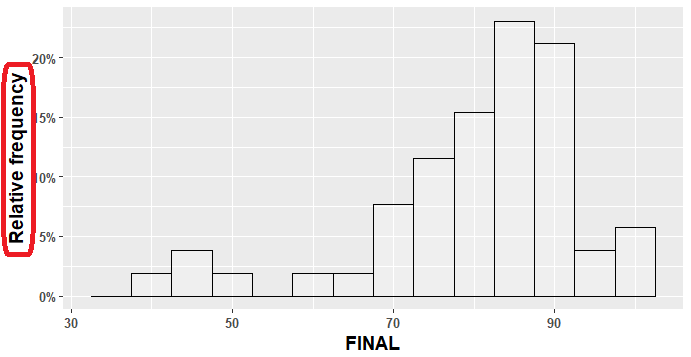
\includegraphics[scale=0.4]{Histogram2.png}
\caption{Histogram of with vertical axis \textbf{relative frequency}}
\label{HistogramRelativeFrequency}
\end{figure}


 
\begin{textblock}{4.8}(-3, -4.5) 
   Compare histogram with stemplot. What are the advantages and disadvantages? 
 \end{textblock}


\item \textbf{Density curve}\vspace{0.3cm}

In figure \ref{HistogramRelativeFrequency}, we can tell the percentage of \textit{FINAL} $\leq 50$ is approximately $8\%$ by adding up the percentages of the first three columns. Here, the percentages are indicated by the height of the bars. (4 out of 52 students with \textit{FINAL} $\leq 50 $. Those values are 42, 47, 47, 49. ). If the histogram is with bin width 1(figure \ref{HistogramBinWidth1}),  the percentage a bar takes can be calculated by
$$\textbf{percentage} = \textbf{bar height} = \textbf{bin width} * \textbf{bar height} = \textbf{area of the bar}.$$

\begin{figure}[H]
\centering
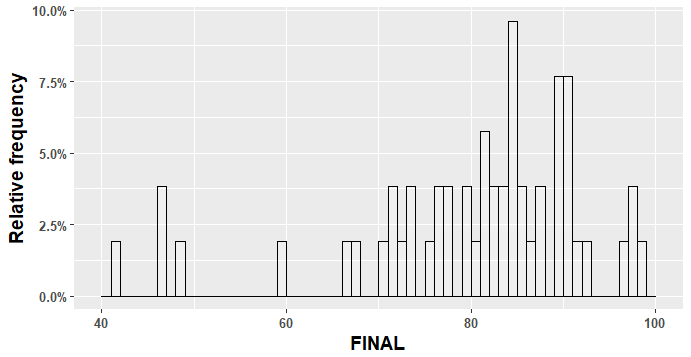
\includegraphics[scale=0.45]{Histogram3.png}
\caption{Histogram  with bin width 1}
\label{HistogramBinWidth1}
\end{figure}
To calculate the percentage of the students with \textit{FINAL}$\leq 50$, just add up the areas of the three bars to the left side of 50. 

\begin{textblock}{4.8}(-3, -5.5)
What is the total area of all bars in figure \ref{HistogramBinWidth1}.
\end{textblock}

Take a step further. A smooth curve can be drawn such that the area to the left side of $\mathbf{x}$ gives the percentage of the number of individuals $\leq \mathbf{x}$.This graph is called \textbf{density curve}. The function of the density curve is called the \textbf{probability density function(pdf)}.
\begin{figure}[H]
\centering
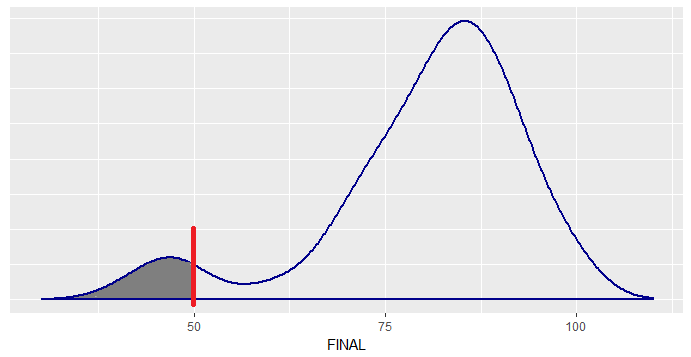
\includegraphics[scale=0.45]{DensityCurve.png}
\caption{Smoothed density curve  of the \textit{FINAL}}
\label{DensityCurve}
\end{figure}
In figure \ref{DensityCurve} , the shaded area gives the percentage of \textit{FINAL}$\leq 50$, which is approximately $8\%$.\vspace{0.3cm}\\
\colorbox{babypink}{\parbox{14.2cm}{Sometimes the vertical axis is suppressed, because it doesn't mean too much in this book.}}\vspace{0.3cm}\\
\begin{textblock}{4.8}(13, -7)
 What is the total area under the density curve?
\end{textblock}

 \item \textbf{Cumulative relative frequency curve}\vspace{0.3cm}
 
In figure \ref{DensityCurve}, for each value of $\mathbf{x}$ there is an area to the left side of this value. Therefore we can get a function $F$,such that 
$$F(x) = \textbf{Area to the left of } \mathbf{x}.$$
If we draw a smooth graph of $F(x)$, it will be like figure \ref{CumulativeRFCurve}. This curve is called the \textbf{cumulative relative frequency curve.} Function $F(x)$ is called \textbf{cumulative distribution function(cdf)}.

\begin{figure}[H]
\centering
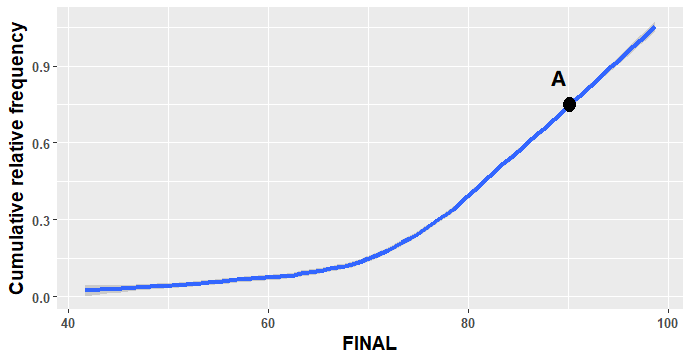
\includegraphics[scale=0.5]{CumulativeRFCurve.png}
\caption{Cumulative relative frequency curve of \textit{FINAL}}
\label{CumulativeRFCurve}
\end{figure}
 
\begin{textblock}{4.8}(13, -6)
How to interpret point \textbf{A} in figure \ref{CumulativeRFCurve}?
\end{textblock}

\begin{textblock}{4.8}(13, -4)
 What is the theoretical relation between a density curve  and its cumulative relative frequency curve?
\end{textblock}
\newpage
\item \textbf{Shape, center and spread of the  graphs}\vspace{0.3cm}

\textbf{Shape} describes the general outlook of the distribution, by describing \textbf{Skewness, clusters, gaps} and \textbf{outliers}.

\begin{figure}[H]
\centering
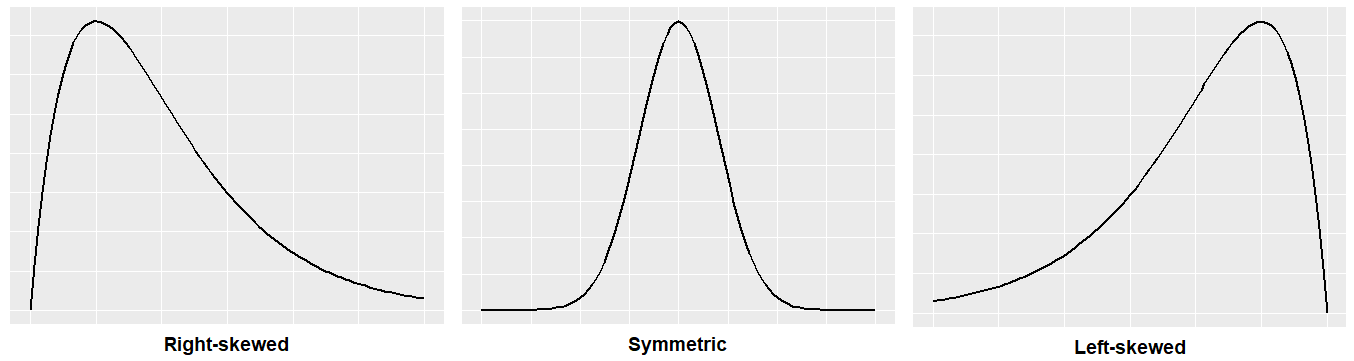
\includegraphics[scale=0.3]{Skewness.png}
\caption{Shapes of distributions}
\label{Skewness}
\end{figure}
As shown in figure \ref{Skewness}, the skewness  of the distributions are \textbf{right-skewed, symmetric} and \textbf{left-skewed} respectively.

\begin{figure}[H]
\centering
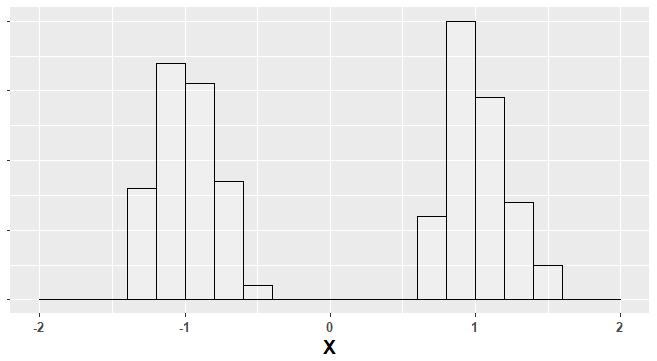
\includegraphics[scale=0.3]{TwoClusters.png}
\caption{Two clusters and a gap}
\label{TwoClusters}
\end{figure}
As show in figure \ref{TwoClusters}, we say the distribution has two \textbf{clusters(modes)} with a \textbf{gap}.

\begin{figure}[H]
\centering
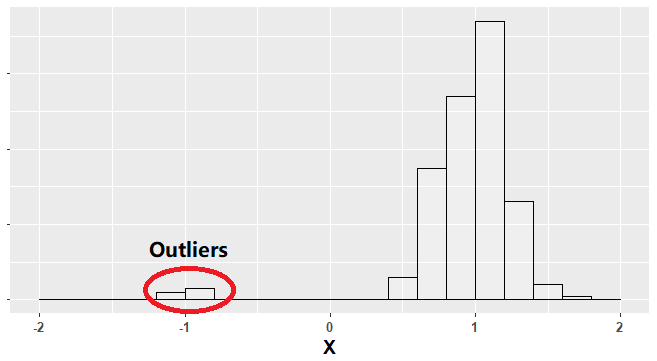
\includegraphics[scale=0.3]{Outliers.png}
\caption{Outliers}
\label{Outliers}
\end{figure}

If some values have striking departures from the pattern of the majority, those values are called \textbf{outliers}(as shown in figure \ref{Outliers}).
 
\colorbox{babypink}{\parbox{14cm}{Outliers need special attention, for they may be generated by mistakes or some other unconsidered mechanisms.}}\vspace{0.6cm}

\textbf{Center} describe the value around which the data is distributed. It will be introduced later\vspace{0.6cm}

\textbf{Spread} describes how widely the data are scattered. It will be learned latter.
\end{itemize}
\newpage


\section{Summarizing distributions}

\begin{itemize}


\item \textbf{Center}\vspace{0.3cm}

There are different ways to describe the center of a distribution. Here we only consider two primary ways of denoting the center:\textbf{median} and \textbf{mean}.\vspace{0.6cm}

 \textbf{Median}\vspace{0.3cm}
 
 Arrange the data in increasing or decreasing order, median is the middle one or the average of the middle two. \vspace{0.6cm}
 
 \textbf{Mean}\vspace{0.3cm}
 
 For data set $\{x_1, x_2, \cdots, x_n\}$, the mean $\bar{x}$ is given by 
 $$\bar{x} = \frac{x_1+x_2+\cdots+x_n}{n}
           = \frac{\sum_{i=1}^{n}x_i}{n} $$

\colorbox{babypink}{\parbox{0.9\textwidth}{Notation $\mu$ is used for population mean and  $\bar{x}$ is for sample mean, though the formulas for them are the same. }}

For example, we draw a sample of 100 students from a high school, and the mean weight of the whole high school is 65kg,  and the mean weight of the 100 students is 60kg. We say
$$\mu = 65 \text{kg}, \quad \overline{x} = 60 \text{kg}.$$

\textbf{Median is resistant}\vspace{0.3cm}

For data $\{1, 2, 3, 4, 5\}$, both the mean and the median are 3. If 5 is changed into 500, the mean is 102, while the median is still the same. Median is not easily influenced by extreme values, it is \textbf{resistant}\vspace{0.6cm}

\textbf{Mean, median and skewness}
\begin{figure}[H]
\centering
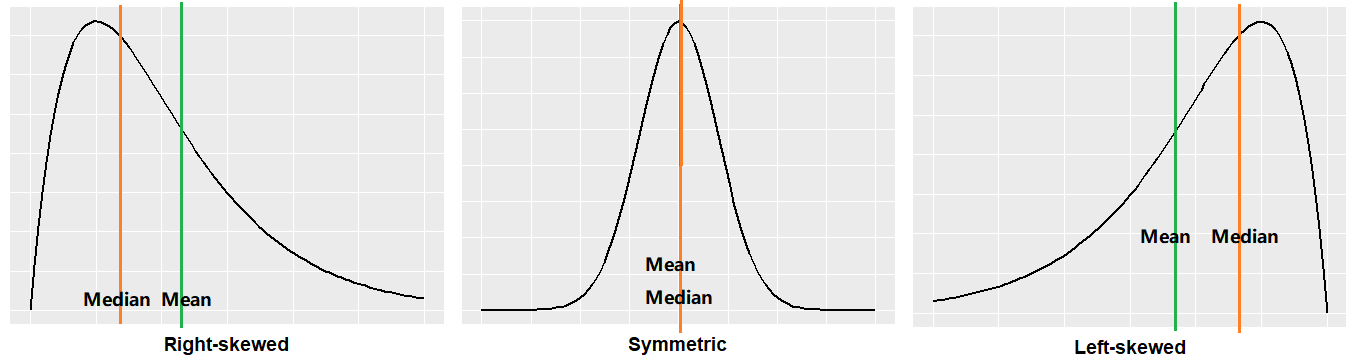
\includegraphics[scale=0.3]{MeanMedian.png}
\caption{The relationship between mean and median}
\label{MeanMedian}
\end{figure}
Generally speaking
 $$\textbf{symmetric distribution} \implies \textbf{mean} = \textbf{median}$$ 
  $$\textbf{right-skewed distribution}\implies \textbf{mean} > \textbf{median}$$
   $$\textbf{left-skewed distribution}\implies \textbf{mean} < \textbf{median}$$

\colorbox{babypink}{\parbox{14.2cm}{If a distribution is strongly skewed, it is better to use the \textbf{resistant} measurement to describe the distribution.}}

\begin{textblock}{4}(14.5, -5)
 Is mean or median a better description of the center of the distribution of personal incomes, which is strongly right-skewed?
\end{textblock}
\newpage

\item \textbf{Spread} \vspace{0.3cm}

\textit{Spread} is to measure the variability or the dispersion of the data. It can be \textbf{range, IQR, variance, standard deviation}.\vspace{0.6cm}

\textbf{Range}
 $$\textbf{range} = \textbf{maximun} -\textbf{minimum}$$\vspace{0.6cm}
 
\textbf{Interquartile range(IQR)}\vspace{0.3cm}

\textbf{First quartile($Q_1$)} is the value with one quarter of the data less than(or equal) to it. For data $\{1,2,3,4,5,6,7,8\}$, 2 is the first quartile.\vspace{0.3cm}

\textbf{Third quartile($Q_1$)} is the value with $3/4$ of the data less than(or equal) to it. For data $\{1,2,3,4,5,6,7,8\}$, 6 is the third quartile.
$$\textbf{IQR} = Q_3 - Q_1$$
\vspace{0.6cm}
\begin{textblock}{4}(-3, -2)
Find the \textit{interquartile range} of\\ $\{1,2,3,4,5,6,7,8\}$
\end{textblock}
\textbf{Variance(Var)}

$$\textbf{Population variance}\quad \textbf{Var}=\sigma^2=\frac{\sum_{i=1}^{n}(x_i-\mu)^2}{n}.$$

$$\textbf{Sample variance}\quad \textbf{Var}=s_x^2=\frac{\sum_{i=1}^{n}(x_i-\bar{x})^2}{n-1}.$$\vspace{0.6cm}

\textbf{Standard deviation}\vspace{0.3cm}

\begin{textblock}{4}(-3, -4.2)
 Calculate the mean, the variance and the standard deviation of sample data $\{1, 2, 3\}$ by hand.
\end{textblock}

\begin{textblock}{4}(-3, 0.5)
What is the unit of the standard deviation?
\end{textblock}

$$\textbf{Population standard deviation}\hspace{0.5cm}\sigma=\sqrt[]{\frac{\sum_{i=1}^{n}(x_i-\mu)^2}{n}}.$$
$$\textbf{Sample standard deviation}\hspace{0.5cm}\bar{x}=\sqrt[]{\frac{\sum_{i=1}^{n}(x_i-\bar{x})^2}{n-1}}.$$

\vspace{0.6cm}

\colorbox{babypink}{\parbox{0.9\textwidth}{Standard deviation is interpreted as the average distance of the data from the mean. It has the same unit as the original data.}}

\begin{textblock}{4}(-3, 0)
\textblockcolor{dollarbill}
Calculate the standard deviation of the \textit{FINAL} in table \ref{ExampleData} by calculator and interpret it.
\end{textblock}

\newpage

\item \textbf{Location}\vspace{0.3cm}

\textbf{Percentile}\vspace{0.3cm}

$n^{th}$ percentile is the value with n percent of the data smaller or equal to it. For data $\{1, 2, 3, 4, 5, 6, 7, 8, 9, 10\}$, 1 is the $10^{th}$ percentile, 6 is the $60^{th}$ percentile.
\begin{textblock}{3}(15.5, -4)
 What percentiles are $Q_1$, median and $Q_3$?
\end{textblock}

\begin{textblock}{3}(15.5, -1.8)
What percentile is the \textit{FINAL} of Vince? Interpret.
\end{textblock}
\vspace{0.6cm}

\textbf{Five number summary}\vspace{0.3cm}

There are five important locations for a given set of data, they are \textbf{min}, $\mathbf{Q_1}$, \textbf{median}, $\mathbf{Q_3}$ and \textbf{max}. They are called a \textbf{five number summary}. The following is a five number summary of the \textit{FINAL} in table \ref{ExampleData}.
\begin{center}
\definecolor{shadecolor}{rgb}{0.969, 0.969, 0.969}\color{fgcolor}\begin{kframe}
\begin{verbatim}
##    Min.     Q1.   Median     Q3.    Max. 
##   42.00   75.50   83.50    90.00   99.00
\end{verbatim}
\end{kframe}
\end{center}
\vspace{0.3cm}

\textbf{1.5 IQR rule}\vspace{0.3cm}

This is rule of thumb to tell whether a value is an outlier or not. 
$$x \notin [Q_1-1.5 \times IQR,\; Q_3+1.5 \times IQR] \implies \text{x is an outlier}.$$

\begin{textblock}{3.6}(15, -2)
\textblockcolor{dollarbill}
Find out the outliers of the \textit{FINAL} by the 1.5 IQR rule.
\end{textblock}
\vspace{0.3cm}

\textbf{Boxplot(box-whisker plot)}
\begin{figure}[H]
\centering
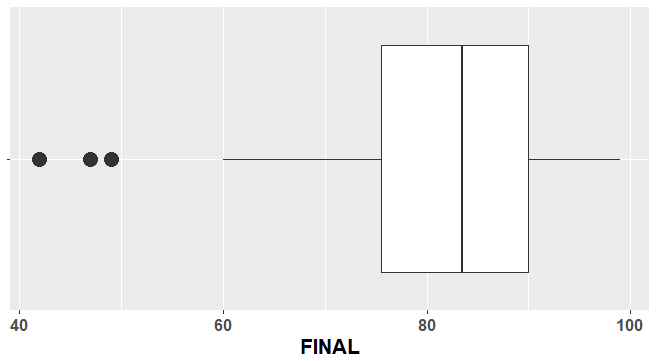
\includegraphics[scale=0.4]{Boxplot.png}
\caption{The boxplot of the \textit{FINAL}}
\label{Boxplot}
\end{figure}
In figure \ref{Boxplot}, the three dots are outliers, the left vertical line of the box indicates the value of the $Q_1$, the middle vertical line indicates the median and the right vertical line indicates the $Q_3$.
\begin{textblock}{4.8}(13.5, -5.5)
 Can you tell the IQR of the \textit{FINAL} according to figure \ref{Boxplot}?
\end{textblock}
\vspace{0.6cm}

\textbf{z-score}\vspace{0.3cm}

For a value $x$, its z-score is given by $$z=\frac{x-\mu}{\sigma} \quad \text{or}\;\; z=\frac{x-\bar{x}}{s_x}.$$
\colorbox{babypink}{\parbox{13.2cm}{The z-score  gives the distance from the mean in terms of standard deviation.}}

\begin{textblock}{4}(14.5, -3.5)
\textblockcolor{dollarbill}
Calculate and interpret the z-score of the \textit{FINAL} of Vince in table \ref{ExampleData}.
\end{textblock}

\end{itemize}
\newpage

\colorbox{champagne}{\parbox{13.2cm}{
\textbf{Exercise:}\vspace{0.3cm}\\
\begin{enumerate}[(1)]
\item 
Find the IQR, median and the skewness of the distribution in figure \ref{Exercise1}.
\begin{figure}[H]
\centering
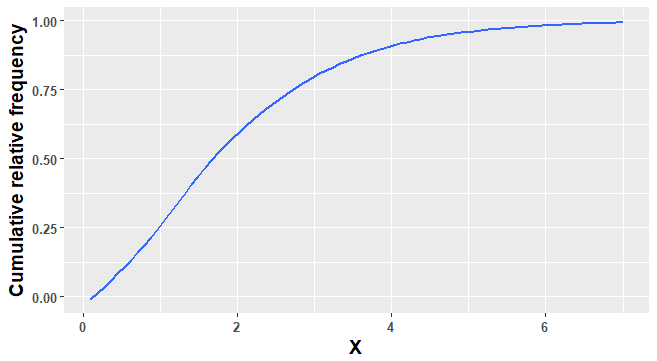
\includegraphics[scale=0.5]{CumulativeSkew.png}
\caption{A cumulative relative frequency curve}
\label{Exercise1}
\end{figure}
\vspace{2cm}

\item In order to select candidates to bid for a government contract on basis of the prices the submitted and rule out those who just mess around, you want to find a range in the form of $[\text{center}-\text{margin}, \text{center}+\text{margin}]$, where the margin is a constant. Any price falls within the range is qualified to be a candidate. Is this center better to be the mean or the median? Why? \vspace{3cm}\\
\item 
Which of the measurements of the spread are resistant?\vspace{2cm}
\end{enumerate}
}}
\newpage
\section{Data transformation}

Suppose we have a sample data set $\mathbf{X} = \{x_1, x_2, \cdots, x_n\}$ with mean $\bar{x}$ and standard deviation $s_x$ . 

\begin{itemize}
\item Add a constant $c$ to the data: 
$\mathbf{X}+c = \{x_1+c, x_2+c, \cdots, x_n+c\}.$
\begin{equation*}
\begin{split}
\text{The mean of}\;\;\mathbf{X}+c &= \frac{(x_1+c)+(x_2+c)+\cdots+(x_n+c)}{n}\\
&= \frac{x_1+x_2+\cdots+x_n}{n}+ c\\
&= \bar{x} + c.
\end{split}
\end{equation*}
\begin{equation*}
\begin{split}
\text{The standard deviation of}\;\;\mathbf{X}+c &= \sqrt{\frac{\sum_{i=1}^n[(x_i+c)-(\bar{x}+c)]^2}{n}}\\
&= \sqrt{\frac{\sum_{i=1}^n(x_i-\bar{x})^2}{n}}\\
&= s_x.
\end{split}
\end{equation*}

\begin{textblock}{4.5}(14, -3)
What about the \textbf{IQR}, \textbf{range} and \textbf{percentiles} if the data is added by a constant c.
\end{textblock}
\hspace{0.3cm}

\item Multiply the data by constant $a$: 
$a\mathbf{X} = \{ax_1, ax_2, \cdots, ax_n\}.$
\begin{equation*}
\begin{split}
\text{The mean of}\;\;\mathbf{aX} &= \frac{(ax_1)+(ax_2)+\cdots+(ax_n)}{n}\\
&= a\frac{x_1+x_2+\cdots+x_n}{n}\\
&= a\bar{x}.
\end{split}
\end{equation*}
\begin{equation*}
\begin{split}
\text{The standard deviation of}\;a\mathbf{X}&= \sqrt{\frac{\sum_{i=1}^n(ax_i-a\bar{x})^2}{n}}\\
&= |a|\sqrt{\frac{\sum_{i=1}^n(x_i-\bar{x})^2}{n}}\\
&= |a|s_x.
\end{split}
\end{equation*}
\end{itemize}

\begin{textblock}{4.5}(14, -5)
\textblockcolor{dollarbill}
Calculate the mean and standard deviation of the z-scores for any give data set.
\end{textblock}

\colorbox{babypink}{\begin{minipage}{0.9\textwidth}
The \textbf{z-score} is also called \textbf{standardized score} for the reason of its mean and standard deviation.\textbf{ It gives us a reasonable way to compare values from different datasets as well.} For example, you get a 4 in \textbf{AP statistics} test and 100 in \textbf{TOEFL} test. Which score is better?  You can compare the z-scores of those two. 
\end{minipage}
}
\newpage

\colorbox{champagne}{\parbox{15.2cm}{
\textbf{Exercise:}\vspace{0.3cm}\\
The height distribution of a class in inches is given below in table  \ref{Heightdistribution}. 
\begin{table}[H]
\centering
\begin{tabular}{c|cccccccc}
Variable&$n$&$\bar{x}$&$S_x$&Min&$Q_1$&Med&$Q_3$&Max\\
\hline
Height&25&67&4.29&60&63&66&69&75\\
\end{tabular}
\caption{Height distribution in inches}
\label{Heightdistribution}
\end{table}
\begin{enumerate}[(1)]
 \item Suppose you convert the class's height form inches to centimeters(1 inch = 2.54 cm). Describe the effect this will have on the shape of the distribution and the values of the variables in table \ref{Heightdistribution}?
 \item If all the students stand on a 6-inch-high platform and them measure the distance from the top of the heads to the ground, how would the shape compare with the original height  distribution and what is the effect on the the values of the variables in table \ref{Heightdistribution}?
 \item Convert all the height to their z-scores, what would this effect the shape of the distribution and the values of the variables in table \ref{Heightdistribution}?
\end{enumerate}
}}

\newpage

\section{Normal distribution}
The \textbf{normal distribution} is one of the most important distributions in statistics. A lot of natural phenomena follow the normal distribution, such as the error of repeated measurements. The \textbf{central limit theorem} makes it more powerful, which says: the sampling distribution of sample mean approaches normal distribution as the sample size increases. Normal distribution is also called \textbf{Gaussian distribution}.
\vspace{0.6cm}

\begin{figure}[H]
\centering
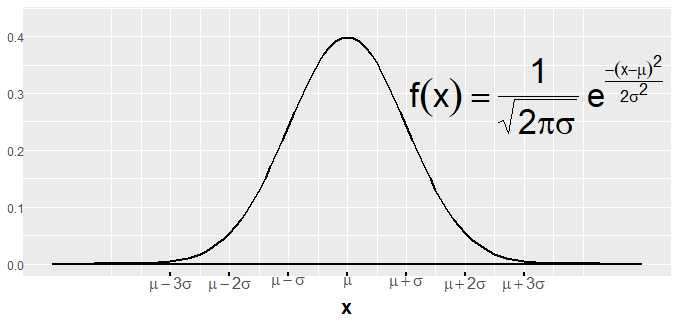
\includegraphics[scale=0.6]{NormalDistribution.png}
\caption{Normal Distribution with mean $\mu$ and standard deviation $\sigma$}
\label{NormalDistribution}
\end{figure}

\begin{itemize}
\item \textbf{Notation}\vspace{0.3cm}\\
Figure \ref{NormalDistribution}, gives the density curve of a normal distribution with mean $\mu$ and standard deviation $\sigma$, and the normal distribution is completely decided by those two parameters. $\mathcal{X}$ follows a normal distribution with mean $\mu$ and standard deviation $\sigma$ is denoted as $\mathcal{X}\sim \mathcal{N}(\mu, \sigma)$.
\vspace{0.6cm}

\item \textbf{The 68-95-99.7 rule}\vspace{0.3cm}\\
The density curve of the normal distribution is symmetric and bell-shaped, with mean equal to median. The total area under the curve and above the horizontal axis is 1. There is an empirical rule for the areas as shown in figure \ref{68-95-99.7Rule}. It is called the \textbf{The 68-95-99.7 rule}.

\begin{figure}[H]
\centering
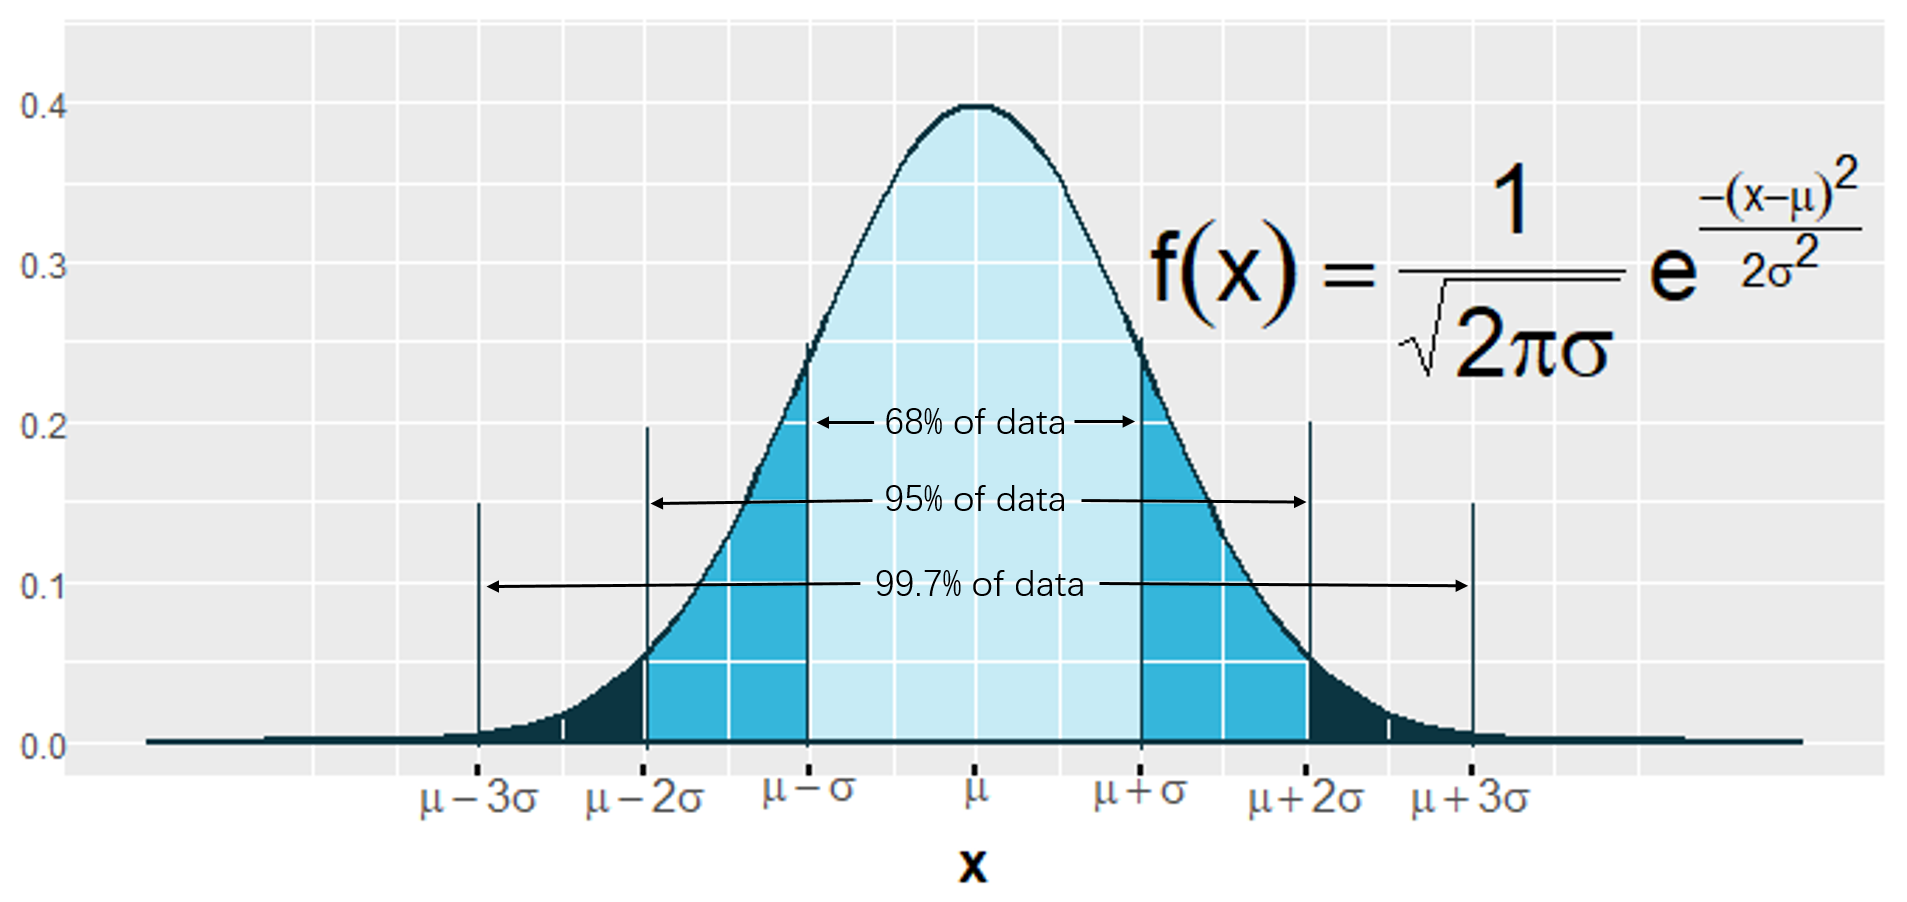
\includegraphics[scale=0.35]{68-95-997Rule.png}
\caption{The 68-95-99.7 rule}
\label{68-95-99.7Rule}
\end{figure}
\colorbox{babypink}{\parbox{\textwidth}{We can estimate the parameters of $\mu$ and $\sigma$ of the normal distributions by the 68-95-99.7 rule.}}

\item \textbf{Standard normal distribution}
\vspace{0.6cm}

Suppose $X \sim \mathcal{N}(\mu, \sigma)$, Let $Z$ be the set of all z-scores of $X$
$$Z=\frac{X - \mu}{\sigma}. $$
Then $Z$ is normally distributed, with mean $\mu_Z$ and standard deviation $\sigma_Z$. According to the knowledge of data transformation: $\mu_Z = 0$, $\sigma_Z = 1$. Thus, $$Z \sim \mathcal{N}(0, 1)$$
$\mathcal{N}(0, 1)$ is called \textbf{standard normal distribution}.
\vspace{0.6cm}

%\begin{textblock}{4}(-3.5, 0)
%$X \sim \mathcal{N}(1,2)$.\\
% find out $P(x<2)$ and $P(0<x<2)$.
%\end{textblock}

Suppose the percentage of the data less than $x$ is give by $P(X<x)$, which equals to the area to the left side of $x$ under the density curve. We have the following equations:
$$P(X<x)= P(\frac{X-\mu}{\sigma}<\frac{x-\mu}{\sigma}) = P(Z<z_x).$$



\colorbox{babypink}{\parbox{14.2cm}{If we known the standard normal distribution of $Z$, we know all the normal distributions.}}
\end{itemize}
\vspace{0.6cm}

 \begin{center}
\textbf{\Large{Normal distribution is very important!!}}
\end{center}
\newpage

\colorbox{champagne}{\begin{minipage}{\textwidth}
\textbf{Exercise}

The amount of time required for each of 100 mice to navigate through a maze was recorded. The histogram below shows the distribution of times, in seconds, for the 100 mice.
\begin{figure}[H]
\centering
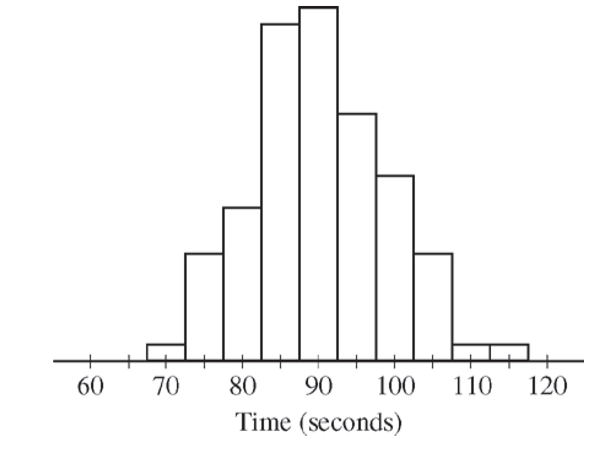
\includegraphics[scale=0.6]{Exercise1.png}
\end{figure}
 Which of the following values is closest to the standard deviation of the 100 times? 
 \begin{enumerate}[(a), start =1]
 \item 2.5 seconds
 \item 10 seconds
 \item 20 seconds
 \item 50 seconds
 \item 90 seconds
 \end{enumerate}
 \end{minipage}
 }
\vspace{0.6cm}


\colorbox{champagne}{\begin{minipage}{\textwidth}
\textbf{Exercise:}

At some fast-food restaurant, customers who want a lid for their drinks get them from a large stack left near straws, napkins, and condiments. The lids are made with small amount of flexibility so they can be stretched across the mouth of the cup and then snugly secured. When lids are too small or too large, customers can get very frustrated especially if the end up spilling their drinks. At one particular restaurant, large drink cups require lids with a "diameter" of between 3.95 and 4.05 inches. The restaurant's lid supplier claims that the diameter of their large lids follows a Normal distribution with mean 3.98 inches and standard deviation 0.02 inches. Assume that the supplier's claim is true.
\begin{enumerate}[(a), start = 1]
\item Find the percentage the large lids are too small to fit.
\item Find the percentage the large lids are too big to fit.
\end{enumerate}
The supplier is considering two changes to reduce the percent of its large-cup lids that are too small to $1\%$. One strategy is to adjust the mean diameter. The other is to alter the production process, thereby decreasing the standard deviation of the lid diameters.
\begin{enumerate}[(a), resume]
\item If the standard deviation remains at $\sigma = 0.02$ inches, at what value should the supplier set the mean diameter of its large-cup lids so that only $1\%$ are too  small to fit?
\item If the mean diameter stays at $\mu = 3.98$ inches, what value of the standard deviation will result in only $1\%$  of lids that are too small to fit?
\item Which of the two options in (c) and (d) do you think is preferable?
\end{enumerate}
\end{minipage}
}
\newpage
\colorbox{champagne}{
\begin{minipage}{\textwidth}
 \textbf{2011FR1}\\
 A professional sports team evaluates potential players for a certain position based on two main characteristics, speed and strength.
   \begin{enumerate}[label = (\alph* )]
      \item Speed is measured by the time required to run a distance of 40 yards, with smaller times indicating more desirable (faster) speeds. From previous speed data for all players in this position, the times to run 40 yards have a mean of 4.60 seconds and a standard deviation of 0.15 seconds, with a minimum time of 4.40 seconds, as shown in the table below.
      \begin{center}
        \begin{tabular}{|c|c|c|c|}
        \hline
         &Mean&Standard Deviation & Minium\\
         \hline
         Time to run 40 yards &$4.60$ seconds &$0.15$ seconds&$4.40$ seconds\\
        \hline
        \end{tabular}
      \end{center}
      
Based on the relationship between the mean, standard deviation, and minimum time, is it reasonable to believe that the distribution of 40-yard running times is approximately normal? Explain.

   \item  Strength is measured by the amount of weight lifted, with more weight indicating more desirable (greater) strength. From previous strength data for all players in this position, the amount of weight lifted has a mean of 310 pounds and a standard deviation of 25 pounds, as shown in the table below.
        \begin{center}
          \begin{tabular}{|c|c|c|}
          \hline
          &Mean&Standard Deviation\\
          \hline
          Amount of weight lifted& $310$ pounds&$25$ pounds\\
          \hline
          \end{tabular}
        \end{center}
       Calculate and interpret the z-score for a player in this position who can lift a weight of 370 pounds.
       
   \item The characteristics of speed and strength are considered to be of equal importance to the team in selecting a player for the position. Based on the information about the means and standard deviations of the speed and strength data for all players and the measurements listed in the table below for Players A and B, which player should the team select if the team can only select one of the two players? Justify your answer
          \begin{center}
             \begin{tabular}{|c|c|c|}
             \hline
             &Player A & Player B\\
             \hline
             Time to run 40 yards & $4.42$ seconds & $4.57$ seconds\\
             \hline
             Amount of weight lifted & $370$ pounds& $375$ pounds\\
             \hline
             \end{tabular}
          \end{center}
   \end{enumerate}
\end{minipage}
}
\newpage

\section{Comparing distributions}
\begin{itemize}
\item \textbf{Perspectives to describe a distribution}\vspace{0.3cm}\\
When you are asked to describe the distribution give by a graph, you are supposed to describe the \textbf{shape, center} and \textbf{spread}. \vspace{0.3cm}\\
For example, by referring to figure \ref{Boxplot}, we say the distribution of the \textit{FINAL} is roughly symmetric, with median around 84, and IQR about 16, and there are 3 outliers.

\item \textbf{Graphs for comparing distributions}\vspace{0.3cm}\\
Many graphs can be drawn to compare the distributions. Figure \ref{BxoplotComparison} and figure \ref{BackToBackSplittingStemPlot} are two of them.
\begin{figure}[H]
\centering
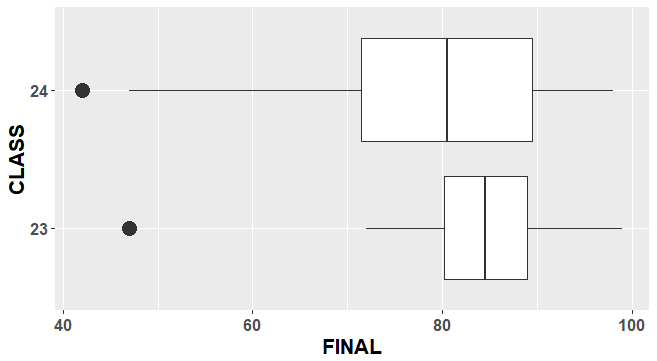
\includegraphics[scale=0.5]{BxoplotComparison.png}
\caption{Distributions of the \textit{FINAL} of \textit{CLASS} 23 and \textit{CLASS} 24}
\label{BxoplotComparison}
\end{figure}

\begin{figure}[H]
\centering
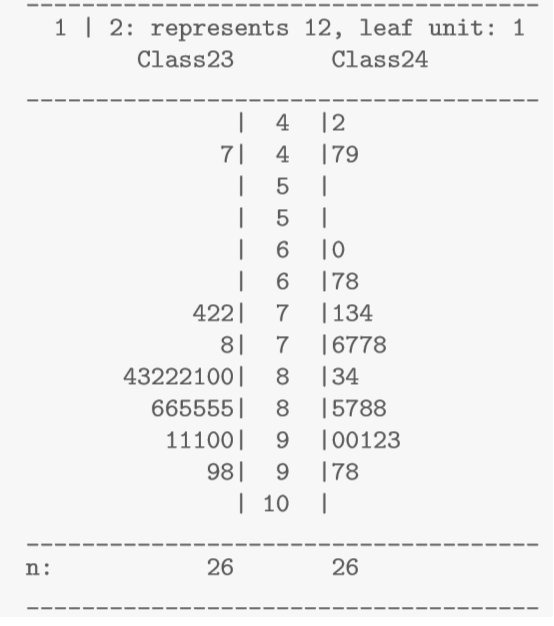
\includegraphics[scale=0.5]{BackToBackSplittingStemPlot.png}
\caption{Back-to-back stem plot with splitting stems}
\label{BackToBackSplittingStemPlot}
\end{figure}


\item \textbf{How to Compare two distributions?}

 The distributions are compared through \textbf{shape, center} and \textbf{spread}, and use proper terms for each perspective.
 \begin{itemize}
 \item For shape, we use terms: \textbf{right-skewed, symmetric, left-skewed, outliers, gaps clusters}.
 \item For center, we use terms:  \textbf{mean} and \textbf{median}.
 \item For spread, we use terms: \textbf{range, IQR} and \textbf{standard deviation}. 
 \end{itemize}
 \end{itemize}
 \newpage

\colorbox{babypink}{\parbox{\textwidth}
{\textbf{\large{Distribution comparison or distribution description problems always show up in AP exam!!}} }}
\vspace{0.6cm}

\colorbox{champagne}{
\parbox{\textwidth}{
\textbf{The "read the graph ans say something" problem}\vspace{0.6cm}\\
Compare the distributions of \textit{FINAL} between different \textit{CLASS} by referring to figure \ref{BxoplotComparison}.
}}


\end{document}